%% =====================================================================================
%%  Research seminar: "Voting for a consensus with veto rights" (the note, v0.1.1)
%% -------------------------------------------------------------------------------------
%%  Build:   cd presentations/draft_research-seminar && latexmk    (writes the PDF next to this file)
%%  Look:    presentations/shared/beamer-style.tex.  Numbers: outputs/tables/key_numbers_en.tex and the
%%           generated tables -- never type a number that the note computes.
%%  About 40 minutes: 25 slides, then backup slides after \appendix.
%%  Never name this file main.tex (on Overleaf the root main.tex would compile instead).
%% =====================================================================================
\documentclass[10pt,aspectratio=169]{beamer}
%% Paths that work whether TeX runs in this folder (local build; Overleaf, which moves to the main
%% document's folder) or at the repository root: files are looked up under each prefix in turn.
\makeatletter
\def\input@path{{../../}{./}}
\makeatother
%% ------------------------------------------------------------------------------------------------
%%  Look shared by the talks of the project (presentations/<talk>/<file>.tex), loaded right after
%%  \documentclass{beamer}. Metropolis theme, in the colours of the figures and the summaries.
%%  Numbers come from outputs/tables/key_numbers_<lang>.tex, figures from outputs/figures/: a talk never
%%  types a number that the note computes. Every talk sits two levels below the repository root; the
%%  paths below work from its folder and from the root (Overleaf).
%% ------------------------------------------------------------------------------------------------
\usetheme[progressbar=frametitle, numbering=fraction, block=fill, sectionpage=progressbar]{metropolis}
\usepackage[T1]{fontenc}
\usepackage{lmodern}
\usepackage{amsmath,amssymb}
\usepackage{booktabs,array}
\usepackage{graphicx}
\graphicspath{{../../outputs/figures/}{outputs/figures/}}

\definecolor{accent}{HTML}{2A78D6}          % slot 1 of the figures' palette, as in the summaries
\definecolor{accentlight}{HTML}{EAF2FC}
\definecolor{ink}{HTML}{0B0B0B}
\definecolor{muted}{HTML}{52514E}
\setbeamercolor{normal text}{fg=ink, bg=white}
\setbeamercolor{alerted text}{fg=accent}
\setbeamercolor{frametitle}{fg=white, bg=ink}
\setbeamercolor{progress bar}{fg=accent, bg=accentlight}
\setbeamercolor{title separator}{fg=accent}
\setbeamercolor{block title}{fg=ink, bg=accentlight}
\setbeamercolor{block body}{fg=ink, bg=accentlight!40}
\setbeamercolor{block title alerted}{fg=white, bg=accent}
\setbeamercolor{block body alerted}{fg=ink, bg=accentlight}
\setbeamertemplate{caption}{\raggedright\insertcaption\par}

%% ---- Notation of the note (manuscript/preamble/macros.tex) --------------------------------------
\newcommand{\sq}{s}
\newcommand{\pref}{\succ}
\newcommand{\Maj}{\operatorname{N}}
\newcommand{\veto}{v}
\newcommand{\Adm}{A_\theta}
\newcommand{\QVC}{\textup{QVC}}
\newcommand{\PVC}{\textup{PVC}}
\newcommand{\conv}{\operatorname{conv}}

%% ---- Slide helpers --------------------------------------------------------------------------------
\newcommand{\src}[1]{{\scriptsize\color{muted}#1}}       % sources of a claim, as author (year)
\newcommand{\yes}{\checkmark}
\newcommand{\no}{$\times$}
%% Generated tables (outputs/tables/*.tex) end with notes written for the note; a talk omits them.
\newsavebox{\tabbox}
\newcommand{\tabnotes}[2]{}
%% \fittables inside a frame: generated tables wider than the slide are scaled down to its width.
\newcommand{\fittables}{\renewcommand{\usebox}[1]{%
  \ifdim\wd##1>\linewidth\resizebox{\linewidth}{!}{\box##1}\else\box##1\fi}}

% Generated by simulations/python/key_numbers.py from outputs/tables/*.csv -- do not edit by hand
\newcommand{\KNdeadlockUnanimity}{99.6}
\newcommand{\KNdeadlockUnanimityEleven}{86}
\newcommand{\KNcontestedSchulze}{10.1}
\newcommand{\KNcontestedQVC}{5.9}
\newcommand{\KNworstoffSchulze}{85.2}
\newcommand{\KNworstoffQVC}{88.4}
\newcommand{\KNworstoffQVCquarter}{92.8}
\newcommand{\KNutilitySchulze}{97.4}
\newcommand{\KNutilityQVC}{97.7}
\newcommand{\KNutilityQVCquarter}{96.8}
\newcommand{\KNcontestedQVCquarter}{5.9}
\newcommand{\KNdeadlockUnanimityPolarised}{97.9}
\newcommand{\KNutilityPlurality}{34}
\newcommand{\KNcondorcetQVC}{94.3}
\newcommand{\KNcondorcetQVCquarter}{83.2}
\newcommand{\KNcondorcetQVCspatial}{99.5}
\newcommand{\KNfallbackQVC}{5.9}
\newcommand{\KNfallbackQVCquarter}{27}
\newcommand{\KNclonesPVC}{54}
\newcommand{\KNclonesBorda}{24}
\newcommand{\KNclonesFallback}{36}
\newcommand{\KNclonesPlurality}{98}
\newcommand{\KNmanipSchulzeSpatial}{5}
\newcommand{\KNmanipSchulzePolarised}{7}
\newcommand{\KNmanipQVCSpatial}{11}
\newcommand{\KNmanipQVCPolarised}{27}
\newcommand{\KNmanipQVCquarterSpatial}{52}
\newcommand{\KNmanipQVCquarterPolarised}{57}
\newcommand{\KNcwPolarisedTwelve}{96}


\title{Voting for a consensus with veto rights}
\subtitle{Open proposals, full ballots and a blocking quota}
\author{Fabrice Borel-Mathurin}
\institute{Research seminar}
\date{Draft, October 2026}

\begin{document}

\maketitle

\begin{frame}{Outline}
  \begin{columns}[T]
    \begin{column}{0.48\textwidth}\tableofcontents[sections={1-4}]\end{column}
    \begin{column}{0.48\textwidth}\tableofcontents[sections={5-7}]\end{column}
  \end{columns}
\end{frame}

%% =============================================================================================
\section{The question}

\begin{frame}{A group must choose one option, by consensus}
  A site, a design, a budget allocation, a policy. Three hypotheses, set by the use case:
  \begin{description}[H1 (open agenda)]
    \item[H1 (open agenda)] anyone may propose as many options as they wish;
    \item[H2 (full ballots)] everyone judges \emph{all} the options proposed;
    \item[H3 (veto rights)] voters can veto.
  \end{description}
  Two requirements:
  \begin{description}[H1 (open agenda)]
    \item[R1] the option chosen is the \alert{best compromise};
    \item[R2] the group \alert{never gets stuck}: the veto must not be too stringent.
  \end{description}
  \medskip
  R1 and R2 pull against each other. Unanimity protects every minority, but one objector blocks
  everything (the \emph{liberum veto}). Majority always decides, but can impose on a large minority.
  \medskip

  \alert{The design question:} how much veto power, held by whom, over what, and how to aggregate the
  rest of the ballot.
\end{frame}

\begin{frame}{The answer in one slide}
  \begin{block}{\QVC($\theta$): Condorcet with a blocking quota, $\theta = 1/3$ by default}
    \begin{enumerate}
      \item Each voter ranks every option and marks the unacceptable ones.
      \item Options vetoed by at least $\theta n$ voters are excluded.
      \item If that excludes every option, the least-vetoed ones are kept.
      \item The Schulze winner among the options left is elected.
    \end{enumerate}
  \end{block}
  \begin{itemize}
    \item Always decides, in one round; the status quo has no default advantage.
    \item The winner is acceptable to more than $1-\theta$ of the voters whenever some option is.
    \item Among acceptable options, the majority decides; adding variants of an option changes nothing.
    \item \alert{The price is strategic vetoing}: a 10\% coalition can manipulate
      \KNmanipQVCSpatial--\KNmanipQVCPolarised\% of structured elections, against
      \KNmanipSchulzeSpatial--\KNmanipSchulzePolarised\% under Schulze.
  \end{itemize}
\end{frame}

%% =============================================================================================
\section{What no procedure can achieve}

\begin{frame}{Impossibility results fix the margins of the choice}
  \begin{itemize}
    \item \textbf{Manipulation is always possible.} With three options or more, every onto,
      non-dictatorial rule is manipulable \src{Gibbard (1973), Satterthwaite (1975)}. The question is
      how often, by whom, at what cost.
    \item \textbf{The majority principle has a cost.} Every Condorcet-consistent rule violates
      participation with four options or more: the no-show paradox \src{Moulin (1988); tight at 12
      voters, Brandt, Geist \& Peters (2017)}.
    \item \textbf{Majorities can cycle, but rarely do in structured electorates.}
      \begin{itemize}
        \item Impartial culture, large $n$: a Condorcet winner exists with probability 91.2\% for three
          options, 74.9\% for five \src{Guilbaud (1952), Gehrlein \& Fishburn (1976)}.
        \item Our spatial and polarised electorates: at least \KNcwPolarisedTwelve\% even with twelve
          options; real ballots agree \src{Regenwetter et al.\ (2006), Tideman \& Plassmann (2012)}.
      \end{itemize}
      A procedure must handle cycles, but they are the exception.
  \end{itemize}
\end{frame}

\begin{frame}{Proposition 1: majority and minority veto conflict}
  \begin{columns}[T]
    \begin{column}{0.52\textwidth}
      \textbf{Example E1}, 100 voters, status quo $C$:\par\smallskip
      \begin{tabular}{rll}
        \toprule
        Voters & Ranking & Veto \\
        \midrule
        51 & $A \pref B \pref C$ & $C$ \\
        49 & $B \pref C \pref A$ & $A$ \\
        \bottomrule
      \end{tabular}
      \medskip
      \begin{itemize}
        \item $A$ is the Condorcet winner: 51--49 against both.
        \item $B$ is everyone's first or second choice; 49\% rank $A$ last and veto it.
      \end{itemize}
    \end{column}
    \begin{column}{0.44\textwidth}
      \begin{block}{Proposition 1}
        For $m \ge 3$ and $0 < \theta < 1/2$, some profiles have a Condorcet winner vetoed by more than
        $\theta n$ voters while another option is acceptable to all. No rule can both elect the Condorcet
        winner and respect a $\theta$-veto there.
      \end{block}
    \end{column}
  \end{columns}
  \medskip
  \alert{Choosing $\theta$ is choosing between $A$ (majority) and $B$ (compromise).} Majority power and
  veto power trade off across rules \src{Kondratev \& Nesterov (2020)}.
\end{frame}

\begin{frame}{Stability and deadlock are two faces of the veto}
  \begin{itemize}
    \item A stable outcome exists for every profile iff $m$ is below the game's Nakamura number
      \src{Nakamura (1979)}: majority has 3, hence cycles; a veto player has $\infty$, hence stability.
    \item Spatial thresholds: a supermajority above $d/(d+1)$ in $d$ dimensions \src{Greenberg (1979)};
      64\% under concave densities \src{Caplin \& Nalebuff (1988)}. Below them, agenda control can lead the
      vote almost anywhere \src{McKelvey (1976)}.
    \item \alert{But the stable outcome a veto guarantees is the status quo.}
  \end{itemize}
  \begin{block}{Proposition 2 (deadlock under unanimity)}
    Voters prefer options closer to their ideal point $p_i \in \mathbb{R}^d$.
    (i) If $\sq \in \conv(p_1, \dots, p_n)$, no option is preferred to $\sq$ by every voter: unanimity with
    the status quo as default keeps $\sq$, whatever the proposals.
    (ii) If the $p_i$ are i.i.d.\ from a distribution whose support contains a neighbourhood of $\sq$, the
    probability of (i) tends to 1 as $n \to \infty$.
  \end{block}
\end{frame}

\begin{frame}{Deadlock in numbers}
  \begin{columns}[c]
    \begin{column}{0.6\textwidth}
      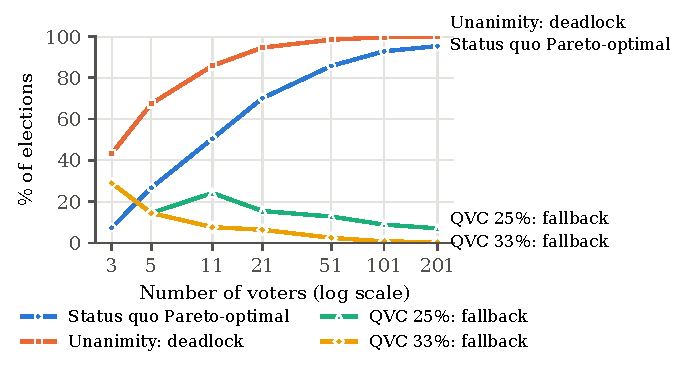
\includegraphics[width=\linewidth]{fig_deadlock}
    \end{column}
    \begin{column}{0.38\textwidth}
      Two dimensions, seven proposals and the status quo. Unanimity keeps the status quo in
      \begin{itemize}
        \item \KNdeadlockUnanimityThree\% of elections with 3 voters,
        \item \KNdeadlockUnanimityEleven\% with 11,
        \item \KNdeadlockUnanimity\% with 101.
      \end{itemize}
      \QVC\ falls back on the least-vetoed options instead, and still decides.
    \end{column}
  \end{columns}
  \medskip
  \src{Buchanan \& Tullock (1962): decision costs rise with the quota. Proposition 2 says they become
  infinite in a large assembly under individual veto.}
\end{frame}

%% =============================================================================================
\section{What research says about veto rights}

\begin{frame}{Unanimity against majority with a veto}
  \begin{itemize}
    \item \textbf{Information aggregation.} Majority rule with a separate veto beats unanimity in large
      committees: a doubter can vote against without blocking \src{Bouton, Llorente-Saguer \& Malherbe
      (2018); laboratory, 2017}.
      \alert{Separate blocking the unacceptable from approving a choice.}
    \item \textbf{Bargaining.} Unanimity brings delay, conflict and surplus captured by holdouts
      \src{Miettinen \& Vanberg (2025), Kagel, Sung \& Winter (2010), Agranov \& Tergiman (2019)}.
    \item \textbf{Veto players.} More veto players, more policy stability, i.e.\ gridlock
      \src{Tsebelis (2002)}; an endogenous status quo adds inertia \src{Dziuda \& Loeper (2016)}; extra
      rounds strengthen the vetoer \src{Nunnari (2021)}.
  \end{itemize}
  \medskip
  Two implications for the design:
  \begin{enumerate}
    \item the status quo must not be a privileged default, or every veto becomes a vote for inertia;
    \item no sequential agenda: the order of votes can be manipulated \src{McKelvey (1976), Barberà \&
      Gerber (2017)}. Under H2, everyone judges all options at once.
  \end{enumerate}
\end{frame}

\begin{frame}{Compromise rules with vetoes, and consensus in practice}
  \begin{columns}[T]
    \begin{column}{0.5\textwidth}
      \textbf{Rules}
      \begin{itemize}\small
        \item Voting by veto \src{Mueller (1978)}
        \item Proportional veto core: $x\%$ of the voters veto $x\%$ of the options
          \src{Moulin (1981, 1982)}; polynomial \src{Ianovski \& Kondratev (2021)}
        \item Fallback bargaining \src{Brams \& Kilgour (2001)}
        \item Majoritarian compromise \src{Sertel \& Yılmaz (1999)}
        \item Shortlisting, veto-rank \src{Barberà \& Coelho (2022), Anbarci (1993)}
      \end{itemize}
      \small Several fail as compromises once the result is known \src{Cailloux, Napolitano \& Sanver
      (2022)}. \alert{None was designed for an open agenda.}
    \end{column}
    \begin{column}{0.48\textwidth}
      \textbf{Practice}
      \begin{itemize}\small
        \item IETF rough consensus: objections addressed, not necessarily accommodated \src{RFC 7282}
        \item Tacit consent: the formal veto is socially constrained \src{Krick (2017)}
        \item \emph{Liberum veto}: paralysis \src{Rohá\v{c} (2008)}
        \item EU Council: a blocking minority needs at least four members \src{TEU, art.\ 16}
        \item \alert{Debian}: ranks all options with ``None of the above''; quorum and majority against the
          default; Schulze. The closest existing procedure, but the default stays privileged.
      \end{itemize}
    \end{column}
  \end{columns}
\end{frame}

\begin{frame}{What the literature supports}
  \footnotesize
  \begin{tabular}{>{\raggedright\arraybackslash}p{0.66\textwidth} l}
    \toprule
    Claim & Evidence \\
    \midrule
    Full unanimity is rarely optimal for open choices: delay, status-quo bias, holdouts & Strong \\
    Majority with a separate veto beats unanimity for information aggregation & Strong \\
    No rule is strategy-proof; the majority principle and minority vetoes conflict & Theorem \\
    One simultaneous ballot removes agenda power; clone independence removes the gain from flooding
      & Strong (theory) \\
    Condorcet winners exist in most structured electorates & Strong \\
    Fallback, shortlisting and veto-rank rules are second-best compromise devices & Moderate \\
    One or two rounds suffice in structured proposal settings & Moderate \\
    In practice, a formal individual veto is socially constrained & Weak to moderate \\
    \bottomrule
  \end{tabular}
  \medskip

  \src{The note, Table 2: adapted and extended from the Consensus review of October 2026.}
\end{frame}

%% =============================================================================================
\section{An open agenda calls for independence of clones}

\begin{frame}{Flooding the agenda}
  \textbf{Clones} are variants of one proposal: no voter ranks another option between them, and every voter
  vetoes all or none \src{Tideman (1987)}. Under H1, anyone can create them.
  \begin{itemize}
    \item Plurality: clones split their supporters' votes and lose. Borda: they push the others down and win.
    \item Independent of clones: Schulze, Ranked Pairs, Split Cycle. Not: Copeland, Minimax, Kemeny--Young.
    \item Veto-based rules are exposed, because $m$ enters their definition: in the proportional veto core,
      each clone the majority adds costs the minority a veto.
  \end{itemize}
  \begin{block}{Proposition 3 (flooding defeats proportional veto)}
    Neither the proportional veto core nor fallback bargaining is independent of clones.
  \end{block}
  In E1, the 49\% block $A$. In \textbf{E2} the majority adds two variants of $A$: the minority's vetoes no
  longer cover them all, and $A$ enters the core and wins.
\end{frame}

\begin{frame}{The rules compared}
  \centering\footnotesize
  \begin{tabular}{l c c c c c}
    \toprule
    Rule & \shortstack{Condorcet\\winner} & \shortstack{Independent\\of clones} & Monotonic & \shortstack{Uses\\vetoes}
      & \shortstack{Never\\stuck} \\
    \midrule
    Plurality              & \no  & \no  & \yes & \no  & \yes \\
    Instant-runoff (IRV)   & \no  & \yes & \no  & \no  & \yes \\
    Borda                  & \no  & \no  & \yes & \no  & \yes \\
    Copeland, Minimax      & \yes & \no  & \yes & \no  & \yes \\
    Schulze, Ranked Pairs, Split Cycle & \yes & \yes & \yes & \no & \yes \\
    Approval               & \no  & \yes$^a$ & \yes & \yes$^b$ & \yes \\
    Fallback bargaining    & \no  & \no  & \yes & \no  & \yes \\
    Unanimity, status quo default & \no & \yes & \yes & \yes & \no \\
    Schulze within the PVC & \no & \no & --- & \yes$^c$ & \yes \\
    \midrule
    \alert{\QVC($\theta$)} & \no$^d$ & \yes & \yes$^e$ & \yes & \yes \\
    \bottomrule
  \end{tabular}
  \raggedright\medskip

  \src{$\times$: fails in some profiles; ---: not established; PVC: proportional veto core. $^a$When clones are approved alike.
  $^b$Non-approval acts as a veto mark but blocks nothing. $^c$Veto power read from the bottom of the
  rankings. $^d$Elects the Condorcet winner of the admissible options (Proposition 6). $^e$For changes in
  the rankings that leave the veto marks unchanged. The note, Table 3.}
\end{frame}

%% =============================================================================================
\section{The procedure: Condorcet with a blocking quota}

\begin{frame}{Six design principles}
  \begin{description}[P1]
    \item[P1] \textbf{One simultaneous ballot} on the whole agenda: no one controls the order of votes.
    \item[P2] \textbf{Ranking and blocking are separate acts}: a ranking plus an acceptability line.
    \item[P3] \textbf{Vetoes are held by coalitions}, a share $\theta$ of the voters, not by individuals.
    \item[P4] \textbf{The status quo is an option like the others}: ranked, vetoed, elected, never the
      default.
    \item[P5] \textbf{The aggregation is clone-independent}: flooding the agenda gains nothing.
    \item[P6] \textbf{A decision is guaranteed}: if every option is blocked, keep the least-vetoed.
  \end{description}
  \medskip
  \src{P1--P2: Bouton et al.\ (2018), McKelvey (1976). P3: Propositions 1--2. P4: Tsebelis (2002), Dziuda \&
  Loeper (2016). P5: Proposition 3. P6: R2.}
\end{frame}

\begin{frame}{\QVC($\theta$)}
  Ballot: a ranking $\pref_i$ with an acceptability line; $V_i$, the options below it. Counts:
  $\veto(x) = |\{i : x \in V_i\}|$ and $\Maj(x,y) = |\{i : x \pref_i y\}|$.
  \begin{block}{Admissible options, $\theta$-compromise}
    $\Adm = \{x : \veto(x) < \theta n\}$ if this set is not empty, else $\arg\min_x \veto(x)$.
    The \emph{$\theta$-compromise} is the Condorcet winner of $\Adm$, when it exists.
  \end{block}
  \begin{enumerate}
    \item Count the vetoes; form $\Adm$ (never empty).
    \item Elect the Schulze winner of $\Adm$. Ties: fewest vetoes, then Schulze on the tied options, then an
      order drawn before the vote.
    \item Publish $\veto$, $\Adm$ and the pairwise matrix $\Maj$, so that anyone can check the count.
  \end{enumerate}
  \medskip
  Lexicographic reading of R1: first acceptable to all but a minority smaller than $\theta$, then majority.
  $O(nm^2 + m^3)$ operations; Ranked Pairs could replace Schulze.
\end{frame}

\begin{frame}{What \QVC($\theta$) guarantees}
  \begin{description}[Prop. 4]
    \item[Prop.\ 4] \textbf{Decisive, with no default advantage.} Exactly one option, in one round, for
      every profile; every option, the status quo included, is treated alike; the order of proposal
      plays no role.
    \item[Prop.\ 5] \textbf{Acceptability.} If some option is vetoed by fewer than $\theta n$ voters, so is
      the winner. No rule elects an option vetoed by a blocking minority less often.
    \item[Prop.\ 6] \textbf{Majority within the admissible options.} The winner is in the Smith set of
      $\Adm$ and not Pareto-dominated; the Condorcet winner of the whole agenda wins whenever fewer than
      $\theta n$ voters veto it.
    \item[Prop.\ 7] \textbf{Independence of clones}, up to the random order that breaks exact ties:
      a clone inherits the vetoes of the original, and Schulze is clone-independent.
  \end{description}
  \medskip
  \src{Proofs: the note, Appendix A. The code checks Propositions 4--7 on random profiles.}
\end{frame}

\begin{frame}{The price: strategic blocking}
  \begin{block}{Proposition 8}
    Any coalition of at least $\theta n$ voters can make any option inadmissible by vetoing it. For every
    $\theta \le 1/2$, there are profiles in which, whatever the winner $w$, at least $\theta n$ voters prefer
    another option to $w$, and can block $w$ although they find it acceptable.
  \end{block}
  \begin{itemize}
    \item The strategic face of Proposition 1: the power to block the unacceptable is also the power to
      block the acceptable.
    \item An option that no coalition of size $\theta n$ wants to replace exists for every profile only if
      $\theta > (m-1)/m$, i.e.\ only if the veto is weaker than majority \src{Greenberg (1979)}.
    \item The proportional veto core avoids the problem, but fails independence of clones
      (Proposition 3), which H1 makes essential.
  \end{itemize}
  \alert{The counting rule cannot remove this; the procedure around the vote must contain it.}
\end{frame}

\begin{frame}{Four worked examples}
  \fittables% Generated by simulations/python/examples.py -- do not edit by hand
\begin{table}[htbp]\centering\footnotesize
\setlength{\tabcolsep}{4pt}
\caption{Winners in the worked examples}\label{tab:examples}
\sbox{\tabbox}{\begin{tabular}{lrrrrrrrrr}
\toprule
Example & Plur. & Borda & Schul. & Fallb. & PVC & Unan. & Q 25\% & Q 33\% & Q 50\% \\
\midrule
E1 (compromise) & A & B & A & B & B & B & B & B & A \\
E2 (flooding) & A & A & A & A & A & B & B & B & A \\
E3 (cycle) & A & A & A & B & A & C (stuck) & B (fb) & A & A \\
E4 (status quo) & X & X & X & Y & X & S (stuck) & X & X & X \\
\bottomrule
\end{tabular}}
\usebox{\tabbox}
\tabnotes{E1: 51 voters rank A, B, C and veto C; 49 rank B, C, A and veto A. E2: E1 after the majority proposes two variants of A, ranked just below A by the majority and last by the minority, which vetoes them. E3: 35 voters rank A, B, C; 33 B, C, A; 32 C, A, B; each bloc vetoes its last option. E4: 99 voters rank X, Y, S and veto S; one voter ranks S, Y, X and vetoes X and Y. The status quo is C in E1--E3 and S in E4. Stuck: no proposal passes and the status quo stays; fb: every option is vetoed by the quota and QVC keeps the least-vetoed ones. Fallb.: fallback bargaining; PVC: Schulze within the proportional veto core; Unan.: unanimity with the status quo as default; Q $x$: QVC with a blocking quota $\theta = x$.}
{Profiles of Section~\ref{sec:examples}; \texttt{examples.py}.}
\end{table}

  \vspace{-0.5em}
  \begin{itemize}\small
    \item \textbf{E1}: the choice of $\theta$ decides between $A$ (majority) and $B$ (compromise).
    \item \textbf{E2}, flooding: Borda, fallback and the proportional veto core switch to $A$; \QVC\ does not
      move.
    \item \textbf{E3}, a cycle: with $\theta = 1/4$ every option is blocked and \QVC\ falls back; with
      $\theta = 1/3$ the weakest option is excluded. Unanimity is stuck.
    \item \textbf{E4}, the status-quo trap: one voter vetoes both proposals; unanimity keeps the status
      quo against 99 voters.
  \end{itemize}
\end{frame}

%% =============================================================================================
\section{Simulation evidence}

\begin{frame}{Design of the Monte Carlo study}
  \begin{itemize}
    \item 101 voters, 8 options: 7 open proposals and the status quo. Proposals are made by voters near
      their own position, so larger blocs propose more and near-duplicates arise, as under H1.
    \item Three electorates: \textbf{spatial} (ideal points on a plane), \textbf{polarised} (two blocs, 55\%
      and 45\%), \textbf{impartial} (random rankings, a worst case).
    \item Vetoes from a personal tolerance fixed before the menu is known: a veto marks the unacceptable,
      not the below-average.
    \item 21 rules, 2,000 elections per electorate. Measures:
      \begin{itemize}\small
        \item Condorcet efficiency; utility and worst-off (10th percentile) efficiency, scaled from 0 for the
          average option to 100 for the best \src{Merrill (1984)};
        \item contested: the winner is vetoed by at least a third; deadlock: the status quo stays;
        \item manipulability by full coalitions and by coalitions of at most 10\% of the voters.
      \end{itemize}
  \end{itemize}
  \src{Every number in the talk comes from the code (\texttt{simulations/python/}), with checks against known
  results.}
\end{frame}

\begin{frame}{Results: the polarised electorate}
  \centering\footnotesize
  \begin{tabular}{l rrrrr}
    \toprule
    Rule & Condorcet eff. & Utility eff. & Worst-off eff. & Contested & Deadlock \\
    \midrule
    Plurality & \KNpolCondPlurality & \KNpolUtilPlurality & \KNpolWorstPlurality & \KNpolContestPlurality & \KNpolDeadPlurality \\
    Borda & \KNpolCondBorda & \KNpolUtilBorda & \KNpolWorstBorda & \KNpolContestBorda & \KNpolDeadBorda \\
    Approval & \KNpolCondApproval & \KNpolUtilApproval & \KNpolWorstApproval & \KNpolContestApproval & \KNpolDeadApproval \\
    Fallback bargaining & \KNpolCondFallback & \KNpolUtilFallback & \KNpolWorstFallback & \KNpolContestFallback & \KNpolDeadFallback \\
    Unanimity, status quo default & \KNpolCondUnanimity & \KNpolUtilUnanimity & \KNpolWorstUnanimity & \KNpolContestUnanimity & \KNpolDeadUnanimity \\
    Schulze & \KNpolCondSchulze & \KNpolUtilSchulze & \KNpolWorstSchulze & \KNpolContestSchulze & \KNpolDeadSchulze \\
    Proportional veto core + Schulze & \KNpolCondPVC & \KNpolUtilPVC & \KNpolWorstPVC & \KNpolContestPVC & \KNpolDeadPVC \\
    \QVC(1/4) & \KNpolCondQVCquarter & \KNpolUtilQVCquarter & \KNpolWorstQVCquarter & \KNpolContestQVCquarter & \KNpolDeadQVCquarter \\
    \alert{\QVC(1/3)} & \alert{\KNpolCondQVCthird} & \alert{\KNpolUtilQVCthird} & \alert{\KNpolWorstQVCthird} & \alert{\KNpolContestQVCthird} & \alert{\KNpolDeadQVCthird} \\
    \bottomrule
  \end{tabular}
  \raggedright\smallskip
  \begin{itemize}\small
    \item Condorcet methods lead on welfare; hard vetoes deadlock.
    \item \QVC(1/3) cuts contested outcomes from \KNpolContestSchulze\% to \KNpolContestQVCthird\%, the minimum any
      rule can reach (Prop.\ 5), and raises worst-off efficiency from \KNpolWorstSchulze\ to
      \KNpolWorstQVCthird, at no cost in total utility. The cost: Condorcet efficiency \KNpolCondQVCthird\%.
  \end{itemize}
  \src{2,000 elections, 101 voters, 8 options; in \%. The note, §7, which also gives the spatial and impartial electorates.}
\end{frame}

\begin{frame}{Flooding and manipulation}
  \begin{columns}[T]
    \begin{column}{0.47\textwidth}
      \textbf{Three clones of a losing option} change the winner in
      \begin{itemize}\small
        \item up to \KNclonesPVC\% of elections: proportional veto core + Schulze;
        \item up to \KNclonesFallback\%: fallback bargaining;
        \item up to \KNclonesBorda\%: Borda (teaming);
        \item \KNclonesSchulze\%: Schulze; \KNclonesQVC\%: \QVC(1/3).
      \end{itemize}
      \small Cloning the winner defeats it under plurality in \KNclonesPlurality\% of spatial elections (vote
      splitting).
    \end{column}
    \begin{column}{0.5\textwidth}
      \textbf{Coalitions of at most 10\% of the voters} can manipulate (spatial--polarised)
      \begin{itemize}\small
        \item Schulze: \KNmanipSchulzeSpatial--\KNmanipSchulzePolarised\%;
        \item \QVC(1/3): \KNmanipQVCSpatial--\KNmanipQVCPolarised\%; \QVC(1/4):
          \KNmanipQVCquarterSpatial--\KNmanipQVCquarterPolarised\%;
        \item instant-runoff: \KNmanipIRVSpatial--\KNmanipIRVPolarised\%; approval:
          \KNmanipApprovalSpatial--\KNmanipApprovalPolarised\%.
      \end{itemize}
      \small Full coalitions manipulate most rules in most elections, \QVC\ with $\theta < 1/2$ in nearly all
      (Prop.\ 8). Three strategies only: lower bounds.
    \end{column}
  \end{columns}
\end{frame}

\begin{frame}{Choosing the quota}
  \centering
  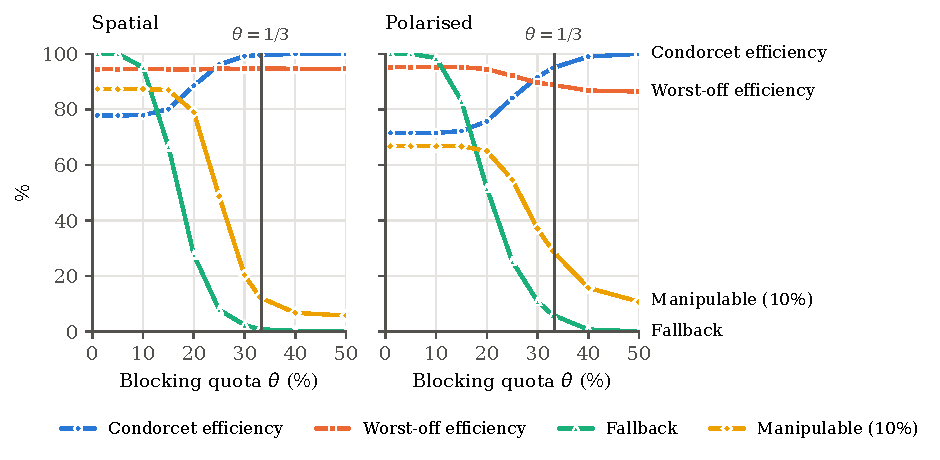
\includegraphics[width=0.66\textwidth]{fig_theta}
  \raggedright\footnotesize
  \begin{itemize}
    \item Low quotas: the fallback decides most elections, the veto is only a negative vote, and the result
      is easily manipulated. High quotas: the veto never binds and \QVC\ is Schulze.
    \item \alert{$\theta = 1/3$}: fallback rare (\KNfallbackQVC\% of polarised elections), Condorcet
      efficiency at least \KNcondorcetQVC\%, most of the worst-off gain kept. Close to the EU's 35\% and to
      the 36\% of the 64\% rule; $\theta = 1/4$ for a group that values consensus more.
  \end{itemize}
\end{frame}

%% =============================================================================================
\section{Safeguards, limits and open questions}

\begin{frame}{Containing strategic vetoes}
  \begin{itemize}
    \item \textbf{Named and reasoned vetoes.} A veto is public and states a reason, as an objection must in
      rough consensus \src{RFC 7282}; responsibility changes votes \src{Breitmoser \& Valasek (2024)}.
    \item \textbf{One revision round, only if the fallback was used.} Nominations reopen briefly for
      compromise proposals; the second ballot is final. One or two rounds suffice; more strengthen
      vetoers \src{Gersbach \& Valkanova (2024), Nunnari (2021)}.
    \item \textbf{Veto budgets across decisions, not within one} \src{storable votes, Casella (2005)}. A
      budget within one decision would break independence of clones.
    \item \textbf{No lower quota than needed}: manipulability falls steeply as $\theta$ rises.
  \end{itemize}
  \medskip
  \src{The status quo can still be protected on purpose, Debian-style, for costly or irreversible decisions.}
\end{frame}

\begin{frame}{How firm, and what is open}
  \begin{columns}[T]
    \begin{column}{0.48\textwidth}
      \textbf{How firm}
      \begin{itemize}\small
        \item Theorems: manipulation is unavoidable; majority and minority veto conflict; unanimity deadlocks
          a large assembly.
        \item Broad literature: Condorcet methods lead on welfare; an open agenda needs clone independence.
        \item Judgement: $\theta = 1/3$. The shape of the trade-off is robust across cultures; the numbers are
          not.
      \end{itemize}
      \textbf{Limits}: one decision; fixed preferences, no deliberation; equal weights; stylised electorates.
    \end{column}
    \begin{column}{0.5\textwidth}
      \textbf{Open questions}
      \begin{itemize}\small
        \item \alert{A clone-proof proportional veto?} Clone independence, veto power proportional to size and
          a non-empty core: compatible, or not?
        \item Fast one- or two-round procedures with hard vetoes in several dimensions.
        \item A strategic comparison of compromise rules under common assumptions.
        \item Do named vetoes reduce strategic blocking? A laboratory test.
        \item Real ballots with acceptability lines: Debian, PrefLib.
      \end{itemize}
    \end{column}
  \end{columns}
\end{frame}

\begin{frame}{Conclusion}
  \begin{itemize}
    \item The research consensus is \alert{negative about unanimity} and positive about vetoes that are
      separate from approval and limited to blocking the unacceptable.
    \item Social choice adds: no escape from manipulation; majority and minority veto must be traded; an
      open agenda requires independence of clones.
    \item One design follows: \alert{\QVC(1/3)}. One ballot; exclude what a blocking third rejects; never
      stuck; Schulze among the rest.
    \item It never deadlocks, protects the worst-off, ignores flooding, and costs no total welfare. Its
      weakness is that of any veto: strategic blocking, to be contained by procedure.
  \end{itemize}
  \vfill
  \begin{center}
    \small Note, code and data: \texttt{github.com/FabriceBM/Vote\_Condorcet}
  \end{center}
\end{frame}

%% =============================================================================================
\appendix

\begin{frame}{Backup: the Schulze method}
  On a set $S$, the link from $x$ to $y$ has strength $d(x,y) = \Maj(x,y)$ if $\Maj(x,y) > \Maj(y,x)$, else
  $0$. The strength $p(x,y)$ of the strongest path is the best, over paths from $x$ to $y$, of the weakest
  link. Floyd--Warshall for widest paths:
  \[
    p(x,y) \gets \max\bigl(p(x,y),\ \min(p(x,z), p(z,y))\bigr) \quad \text{for } z \in S, \text{ then all } x, y,
  \]
  from $p = d$, in $O(|S|^3)$. Winners: the $x$ with $p(x,y) \ge p(y,x)$ for every $y$; there is always one.
  \medskip

  Condorcet- and Smith-consistent, clone-independent, monotonic, Pareto \src{Schulze (2011)}. Used by
  Debian.
\end{frame}

\begin{frame}{Backup: testing the proportional veto core by max-flow}
  $W_i(x)$: the options voter $i$ ranks at or below $x$, $x$ included.
  \begin{block}{Lemma}
    $x$ is in the proportional veto core iff $\bigl|\bigcup_{i \in T} W_i(x)\bigr| \ge m|T|/n$ for every
    coalition $T$; equivalently, the maximum flow equals $mn$ in the network
    \[
      \text{source} \xrightarrow{\;m\;} i \xrightarrow{\;\infty\;} y \in W_i(x) \xrightarrow{\;n\;}
      \text{sink}.
    \]
  \end{block}
  A cut keeping the voters of $T$ on the source side must keep $\bigcup_T W_i(x)$ there; its capacity is
  $m(n-t) + n|\bigcup_T W_i(x)|$. One max-flow per option, on $n + m + 2$ nodes; checked against the
  definition by enumeration on small profiles. \src{Polynomial algorithm: Ianovski \& Kondratev (2021).}
\end{frame}

\begin{frame}{Backup: proof of Proposition 2(i)}
  Suppose $y$ is strictly preferred to $\sq$ by every voter: $\|y - p_i\| < \|\sq - p_i\|$ for all $i$.
  Expanding the squares,
  \[
    (y - \sq) \cdot p_i > \tfrac12\bigl(\|y\|^2 - \|\sq\|^2\bigr) \quad \text{for all } i,
  \]
  so every ideal point lies in an open half-space $H$, which is convex and contains
  $\conv(p_1, \dots, p_n)$. But $\sq \notin H$:
  \[
    (y - \sq) \cdot \sq - \tfrac12\bigl(\|y\|^2 - \|\sq\|^2\bigr) = -\tfrac12\|y - \sq\|^2 < 0.
  \]
  Hence $\sq \notin \conv(p_1, \dots, p_n)$. Under unanimity with the status quo as default, a proposal
  passes only if every voter prefers it to $\sq$, so none passes. \hfill$\square$
  \medskip

  (ii): a small simplex around $\sq$ inside the support; each of its $d+1$ vertex balls receives an ideal
  point with probability $\to 1$.
\end{frame}

\begin{frame}{Backup: putting the procedure to work}
  \begin{enumerate}
    \item \textbf{Fix the parameters in advance}: the quota ($\lceil n/3 \rceil$ voters by default), whether the
      status quo is protected (by default not), the nomination period, the revision round.
    \item \textbf{Nomination}: anyone proposes any number of options; the status quo, or ``none of the
      above'', is on the ballot.
    \item \textbf{Ballot}: rank or grade every option, ties allowed; mark the unacceptable ones; a veto is
      named and reasoned. Grade form: excellent, good, fair, poor, unacceptable.
    \item \textbf{Count} with \QVC; publish the veto counts, the admissible options, the pairwise matrix and
      the winner; anyone can check it with the reference code.
    \item \textbf{Revision round}, only if every option was vetoed by the quota; the second result is final.
  \end{enumerate}
  \medskip
  \src{Small groups: the quota is a number of voters; below five voters, two vetoes, so that no single
  member blocks alone.}
\end{frame}

\begin{frame}{Backup: the simulated electorates}
  \begin{itemize}\small
    \item Proposals: a voter drawn at random proposes an option at their ideal point plus Gaussian noise
      (s.d.\ 0.25); the status quo is drawn independently. Utility: minus the Euclidean distance.
    \item Spatial: ideal points $\sim \mathcal{N}(0, I_2)$. Polarised: blocs of probability 0.55 and 0.45
      centred at $(\pm 1.2, 0)$, s.d.\ 0.6. Impartial: utilities i.i.d.\ uniform.
    \item Vetoes: beyond a personal tolerance, $\rho_i \sim U(1.5, 2.5)$ in distance (spatial cultures),
      fixed before the menu, so clones inherit the original's vetoes.
    \item Efficiency of winner $w$ for a score $S$: $(S(w) - \bar S)/(\max_x S(x) - \bar S)$, $S$ the sum of
      utilities or their 10th percentile across voters.
    \item Manipulation: the voters who prefer $y$ to the winner (all of them, or the first ten) try three
      joint ballots; a success counts. Shares are lower bounds.
    \item Each election has its own seed: the tables are identical from run to run.
  \end{itemize}
  \src{The note, Appendix C; \texttt{cultures.py}, \texttt{voting.py}, \texttt{experiments.py}.}
\end{frame}

\end{document}
